\chapter{Approssimazione di funzioni}

\section{Esercizio 1}
\label{sub:Esercizio 1}
\emph{Sia $f(x) = 4x^{2} - 12x +1$. Determinare $p(x) \in \Pi_{4} $ che interpola $f(x)$ sulle ascisse $x_{i} = i, i = 0, \ldots 4$.}
\begin{sol}
	Caso Lagrange:\\
	Per prima cosa si calcolano gli $f(x_{i})$ per ogni i=0,...,4:\\
	$f(0)=1$\\
	$f(1)=-7$\\
	$f(2)=-7$\\
	$f(3)=1$\\
	$f(4)=17$\\
	Adesso calcoliamo $L_{kn}(x)$ con $k=0,...,4$ e $n=4$:\\
	$L_{04}\frac{(x-1)(x-2)(x-3)(x-4)}{24}$\\
	$L_{14}\frac{(-x)(x-2)(x-3)(x-4)}{6}$\\
	$L_{24}\frac{(x)(x-1)(x-3)(x-4)}{4}$\\
	$L_{34}\frac{(-x)(x-1)(x-2)(x-4)}{6}$\\
	$L_{44}\frac{(x)(x-1)(x-2)(x-3)}{24}$\\

	A questo punto possiamo scrivere $ p(x)\in\Pi_{4} $ = $\frac{(x-1)(x-2)(x-3)(x-4)}{24}$-7$\frac{(-x)(x-2)(x-3)(x-4)}{6}$-7$\frac{(x)(x-1)(x-3)(x-4)}{4}$+$\frac{(-x)(x-1)(x-2)(x-4)}{6}$+17$\frac{(x)(x-1)(x-2)(x-3)}{24}$

	\vspace{2mm}
	Eseguendo i calcoli, si ottiene il polinomio $p(x)=4x^{2}-12x+1$
\end{sol}

\sectionline{black}{88}

\section{Esercizio 2}
\label{sub:Esercizio 2}
\emph{Dimostrare che il seguente algoritmo, \\}
\lstset{language=Matlab}
\begin{lstlisting}
p = a(n+1)
for k = n:-1:1
	p = p*x +a(k)
end
\end{lstlisting}
\emph{valuta il polinomio (4.4) nel punto x, se il vettore $a$ contiene i coefficienti del polinomio $p(x)$ (Osservare che in \textsc{Matlab} i vettori hanno indice che parte da 1, invece che da 0).}
\begin{sol}
	Un polinomio nella base delle potenze è scritto come
	$\sum_{k=0}^{n}a_{k}x^{k}$; raccogliendo di volta in volta una x,
	si ottiene:

		\[a_{0}+a_{1}x+a_{2}x^{2}+...+a_{n}x^{n}=a_{0}+x(a_{1}+a_{2}x+...+a_{n}x^{n-1})=...=
	\]
		\[=a_{0}+x(a_{1}+x(a_{2}+...+x(a_{n-1}+a_{n}x)))
	\]

	L'algoritmo di Horner esegue una somma e un prodotto ad
	ognuno degli n passi, il costo complessivo è, quindi, di $2n$ flops contro
	i $\sum_{i=0}^{n}(i+1)=\frac{(n+1)(n+2)}{2}\approx\frac{n^{2}}{2}$
	flops della valutazione iniziale. Nell'implementazione è possibile
	valutare il polinomio in un insieme di punti, passando un vettore
	di ascisse.
\end{sol}
\sectionline{black}{88}

\section{Esercizio 3}
\label{sub:Esercizio 3}
\emph{Dimostrare il lemma 4.1}
\begin{sol}
	Si distingono due casi. Se $ k=i: \Rightarrow $

		 \[L_{kn}(x_{i})=\prod\limits_{j=0,j\neq{k}}^n {\frac{x_{i}-x_{j}}{x_{i}-x_{j}}} = 1
	 \]

	Se $ k\neq{i}: \Rightarrow $

		 \[L_{kn}(x_{i})=\prod\limits_{j=0,j\neq{k}}^n {\frac{x_{i}-x_{j}}{x_{k}-x_{j}}} = {\frac{x_{i}-x_{0}}{x_{k}-x_{0}}} \text{} ... \text{} {\frac{x_{i}-x_{i}}{x_{k}-x_{i}}} \text{} ... \text{} {\frac{x_{i}-x_{n}}{x_{k}-x_{n}}} =
	 \]
		\[= {\frac{x_{i}-x_{0}}{x_{k}-x_{0}}} \text{} ... \text{} 0 \text{} ... \text{} {\frac{x_{i}-x_{n}}{x_{k}-x_{n}}} = 0
	\]

	\begin{enumerate}
		\item Appare inoltre evidente che il polinomio ha grado esatto n: è il prodotto di (n+1)-1
	fattori $x-x_{j}$ al numeratore (mentre al denominatore abbiamo una quantità costante,
	scelto k). Per quanto riguarda il coefficiente principale, osserviamo che:
		\[
		L_{kn}(x)=\prod\limits_{j=0,j\neq{k}}^n {\frac{(x-x_{j})}{(x_{k}-x_{j})}} = \frac{\prod\limits_{j=0,j\neq{k}}^n {(x-x_{j})}}{\prod\limits_{j=0,j\neq{k}}^n {(x_{k}-x_{j})}} = c_{kn} \text{} \prod\limits_{j=0,j\neq{k}}^n {(x-x_{j})}
	\]
	con
		\[
		c_{kn}=\frac{1}{\prod\limits_{j=0,j\neq{k}}^n {(x_{k}-x_{j})}}
	\]
	costante e diverso da zero per ipotesi.
	\item Gli n polinomi (al variare di k = 1...n) sono tra loro linearmente indipendenti, infatti:
		\[
		a_{1}L_{1n}(x)+ ... +a_{n}L_{nn}(x)
	\]
	si ha che per $x = x_{i}$ tutti i termini della somma si annullano (dalle dimostrazioni precedenti) e rimane soltanto $a_{i}L_{in}(x_{i}) = 0 \Rightarrow a_{i}1 = 0$ e quindi estendendo il ragionamento su tutti gli i = 1...n abbiamo che devono essere nulli i vari $a_{i}$.
	\end{enumerate}
\end{sol}
\sectionline{black}{88}

\section{Esercizio 4}
\label{sub:Esercizio 4}
\emph{Dimostrare il lemma 4.2}
\begin{sol}
	\begin{enumerate}
		\item $w_{k}(x)\in \Pi_{k}\textsuperscript{'}$ è di grado \textit{k}. Infatti:
			\[w_{k}(x)=(x-x_{k-1})\text{}w_{k-1}(x) = (x-x_{k-1})\text{}(x-x_{k-2})\text{}w_{k-2}(x) =\]
		...
			\[= (x-x_{k-1})\text{}(x-x_{k-2})\text{}...\text{}(x-x_{1})\text{}w_{0}(x) = (x-x_{k-1})\text{}(x-x_{k-2})\text{}...\text{}(x-x_{1})\text{}1\]
		Sicuramente il termine di grado più alto del polinomio risultante dal precedente prodotto sarà \textit{k}. Inoltre, tale termine avrà come coefficiente 1.
		\item Il prodotto del punto 1 può anche essere scritto come produttoria, ottenendo, quindi, la tesi:
			\[ w_{k}(x)=\prod\limits_{j=0}^k (x-x_{j}) \]
		\item è sufficiente verificare quanto segue:
			\[
			w_{k+1}(x_{j})=(x_{j}-x_{k})\text{}(x_{j}-x_{k})\text{}...\text{}(x_{j}-x_{j})\text{}...\text{}(x_{j}-x_{1})\text{}1 =
		\]
				\[
			=(x_{j}-x_{k})\text{}(x_{j}-x_{k})\text{}...\text{}0\text{}...\text{}(x_{j}-x_{1})\text{}1 = 0
		\]
		\item Il generico $w_{i}(x)$ è un polinomio monico di grado i e appartiene a $\Pi_{i}$, per cui i polinomi per i = 1...k generano lo spazio $\Pi_{k}$.

	Sia $a_{1}w_{0}(x)+...+a_{k}w_{k}(x)$ una combinazione lineare.
	Questa deve essere banale, poichè, se così non fosse, ci sarebbero alcuni $w_{i}(x)=0$ per ogni ascissa data
	$x_{0},..., x_{n}$; ma, quindi, nella produttoria $\prod\limits_{j=0}^k (x-x_{j}) $
	ci sarebbe un termine nullo per qualsiasi ascissa che consideriamo, ciò comporterebbe che i prodotti sono tutti nulli,
	ma tale asserzione è assurda.
\end{enumerate}
\end{sol}

\sectionline{black}{88}

\section{Esercizio 5}
\label{sub:Esercizio 5}
\emph{Dimostrare il lemma 4.4}
\begin{sol}
	\normalfont
	\begin{enumerate}
		\item Linearità delle differenze divise: \begin{equation*}\begin{split}(\alpha f+\beta g)&[x_0,\ldots,x_r]=\sum_{k=0}^r{\frac{\alpha f_k+\beta g_k}{\prod_{j=0,j\neq k}^r{(x_k-x_j)}}}=\\=&\sum_{k=0}^r{\frac{\alpha f_k}{\prod_{j=0,j\neq k}^r{(x_k-x_j)}}}+\sum_{k=0}^r{\frac{\beta g_k}{\prod_{j=0,j\neq k}^r{(x_k-x_j)}}}=\\=&\alpha\sum_{k=0}^r{\frac{f_k}{\prod_{j=0,j\neq k}^r{(x_k-x_j)}}}+\beta\sum_{k=0}^r{\frac{g_k}{\prod_{j=0,j\neq k}^r{(x_k-x_j)}}}=\\=&\alpha f[x_0,\ldots,x_r]+\beta g[x_0,\ldots,x_r].\end{split}\end{equation*}
		\item La permutazione degli indici è possibile poichè somme e prodotti sono operazioni commutative.
		\item Differenze divise e polinomi: dato che $f(x)$ è un polinomio ed il polinomio interpolante è unico, $$f(x)=\sum_{i=0}^k{a_ix^i}=\sum_{i=0}^k{f[x_0,\ldots,x_k]w_k(x)}=p_k(x).$$Il termine $k$-esimo è $a_kx^k=f[x_0,\ldots,x_k]w_k(x)$ quindi $f[x_0,\ldots,x_k]=a_k$ poiché $w_k(x)\in\Pi'_k$. I termini con $r>k$ non compaiono nella funzione dunque hanno coefficiente $f[x_0,\ldots,x_r]=0$.
		\item Derivabilità: sia $p(x)$ il polinomio interplante allora $e(x)=f(x)-p(x)\in C^{(r)}\left([a,b]\right)$ ed $e(x_i)=0$ per $i=0,\ldots,r$. Per il teorema di Rolle sulle funzioni continue, $\exists\xi^{(1)}_i\in\left[x_i,x_{i+1}\right]$ tali che $e'(\xi^{(1)}_i)=0$ per $i=0,\ldots,r-1$. Reiterando, $\exists\xi^{(2)}_i\in\left[\xi^{(1)}_i,\xi^{(1)}_{i+1}\right]$ tali che $e''(\xi^{(2)}_i)=0$ per $i=0,\ldots,r-2$ e così via; infine $\exists\xi^{(r)}\in\left[a,b\right]$ tali che $e^{(r)}(\xi^{(r)})=0$. Segue $e^{(r)}(x)=f^{(r)}(x)-p^{(r)}(x)=f^{(r)}(x)-r!f[x_0,\ldots,x_r]=0$ ovvero $f[x_0,\ldots,x_r]=\frac{f^{(r)}(\xi^{(r)})}{r!}$.
		\item Ricorsività: \begin{equation*}\begin{split}\:&\frac{f[x_1,\ldots,x_r]-f[x_0,\ldots,x_{r-1}]}{x_r-x_0}=\\=&\left[\sum_{k=1}^r{\frac{f_k}{\prod_{j=1,j\neq k}^r(x_k-x_j)}} + \sum_{k=0}^{r-1}{\frac{f_k}{\prod_{j=0,j\neq k}^{r-1}(x_k-x_j)}}\right]\frac{1}{x_r-x_0} = \\ =&\left[\sum_{k=1}^r{\frac{f_k(x_j-x_0)}{\prod_{j=0,j\neq k}^r(x_k-x_j)}} - \sum_{k=0}^{r-1}{\frac{f_k(x_j-x_k)}{\prod_{j=0,j\neq k}^r(x_k-x_j)}}\right]\frac{1}{x_r-x_0} = \\=&\left[\sum_{k=0}^r{\frac{f_k(x_j-x_0)}{\prod_{j=0,j\neq k}^r(x_k-x_j)}} - \sum_{k=0}^{r}{\frac{f_k(x_j-x_k)}{\prod_{j=0,j\neq k}^r(x_k-x_j)}}\right]\frac{1}{x_r-x_0} = \\=& \left[\sum_{k=0}^r{\frac{f_k(x_j-x_0)-f_k(x_j-x_k)}{\prod_{j=0,j\neq k}^r(x_k-x_j)}}\right]\frac{1}{x_r-x_0}  =\\=&
	\left[\sum_{k=0}^r{\frac{f_k(x_r-x_0)}{\prod_{j=0,j\neq k}^r(x_k-x_j)}}\right]\frac{1}{x_r-x_0}= \\=&(x_r-x_0)\left[\sum_{k=0}^r{\frac{f_k}{\prod_{j=0,j\neq k}^r(x_k-x_j)}}\right]\frac{1}{x_r-x_0}= \end{split}\end{equation*}
	\newpage\begin{equation*}\begin{split}=&\sum_{k=0}^r{\frac{f_k}{\prod_{j=0,j\neq k}^r(x_k-x_j)}} = f[x_0,\ldots,x_r].\end{split}\end{equation*}
	\end{enumerate}
\end{sol}

\sectionline{black}{88}

\section{Esercizio 6}
\label{sub:Esercizio 6}
\emph{Costruire una \lstinline{function} \textsc{Matlab} che implementi in modo efficiente l'Algoritmo 4.1}
\begin{sol}
	\lstinputlisting[caption={Calcolo delle differenze divise.}, label=lst:differenzeDivise]{code/differenzeDivise.m}
\end{sol}
\sectionline{black}{88}

\section{Esercizio 7}
\label{sub:Esercizio 7}
\emph{Dimostrare che il seguente algoritmo, che riceve in ingresso i vettori $x$ e $f$ prodotti dalla \lstinline{function} dell'Esercizio 4.6, valuta il corrispondente polinomio interpolante di Newton in un punto $xx$
assegnato.}\\
\lstset{language=Matlab}
\begin{lstlisting}
  p = f(n+1)
  for k = n:-1:1
  	p = p*(xx-x(k)) +f(k)
  end
\end{lstlisting}
\emph{Quale è il suo costo computazionale? Confrontarlo con quello dell'Algoritmo 4.1. Costruire, quindi, una corrispondente \lstinline{function} \textsc{Matlab} che lo implementi efficientemente (complementare la possibilità che $xx$ sia un vettore)}
\begin{sol}
	Essendo un polinomio in forma di Newton esprimibile come
	$$p_n(x)=\sum_{k=0}^nf[x_0,\dots,x_k]w_k(x)$$
	ed essendo il $(k+1)$-esimo polinomio della base di Newton esprimibile come
	$$w_{k+1}=\prod_{j=0}^k(x-x_j),$$
	vediamo che, come nel caso dell'Esercizio \ref{es4.2}, possiamo raggruppare i vari $(x-x_i)$ e
	considerare le differenze divise come coefficienti rispetto alla base di Newton. Si ottiene quindi:
	\begin{align*}
		\sum_{k=0}^nf[x_0,\dots,x_k]w_k(x) &= f[x_0] +(x-x_0)(f[x_0,x_1]+\dots\\
		&\dots+(x-x_{n-2})(f[x_0,\dots,x_{n-1}]+f[x_0,\dots,x_n](x-x_{n-1}))\dots).
	\end{align*}
	Quindi, eseguendo le operazioni nell'ordine indicato, otteniamo l'algoritmo di Horner generalizzato,
	il cui costo risulta essere di $3n$ \texttt{flop}, in quanto ad ogni iterazione vengono eseguiti una sottrazione,
	un prodotto ed una somma. Il costo dell'Algoritmo per il calcolo delle differenze divise risulta invece essere pari a
	$(\frac{3}{2}n^2-3n)$ \texttt{flop},
	in quanto per calcolare ogni differenza divisa vengono eseguite due sottrazioni ed una divisione ($3$ \texttt{flop})
	ed il numero di differenze divise da calcolare è pari al numero di elementi triangolari inferiori di una matrice $n\times n$ (quindi $\frac{1}{2}n^2$)
	meno gli elementi della prima colonna (che sono $n$) che sono dati.\\
	Nell'implementazione \textsc{Matlab}, proposta di seguito, si è considerato il caso in cui \lstinline{xx} sia un vettore di punti semplicemente reiterando $m$ volte, con $m$ dimensione del vettore \lstinline{xx}, l'algoritmo di Horner generalizzato. in questo caso il costo computazionale risulta essere $3mn$ \texttt{flop}.
	\lstinputlisting[caption={Algoritmo di Horner generalizzato.}]{code/hornerGeneralizzato.m}
\end{sol}

\sectionline{black}{88}

\section{Esercizio 8}
\label{sub:Esercizio 8}
\emph{Costruire una \lstinline{function} \textsc{Matlab} che implementi in modo efficiente l'algoritmo del calcolo delle differenze divise per il polinomio di Hermite.}
\begin{sol}
	\lstinputlisting[caption={Calcolo delle differenze divise per il polinomio di Hermite.}, label=lst:differenzeDiviseHermite]{code/differenzeDiviseHermite.m}
\end{sol}
\sectionline{black}{88}

\section{Esercizio 9}
\label{sub:Esercizio 9}
\emph{Si consideri la funzione
$$f(x)=(x-1)^9.$$
Utilizzando le \lstinline{function} degli Esercizi 4.6 e 4.8, valutare i polinomi interpolanti di Newton e di Hermite sulle ascisse
$$0,0.25,0.5,0.75,1,$$
per x=linspace(0,1,101). Raffigurare, quindi, (e spiegare) i risultati.}

\begin{sol}
	I seguenti grafici mostrano i risultati ottenuti interpolando la funzione sulle ascisse indicate con i polinomi di Newton e di Hermite:
	\begin{center}
		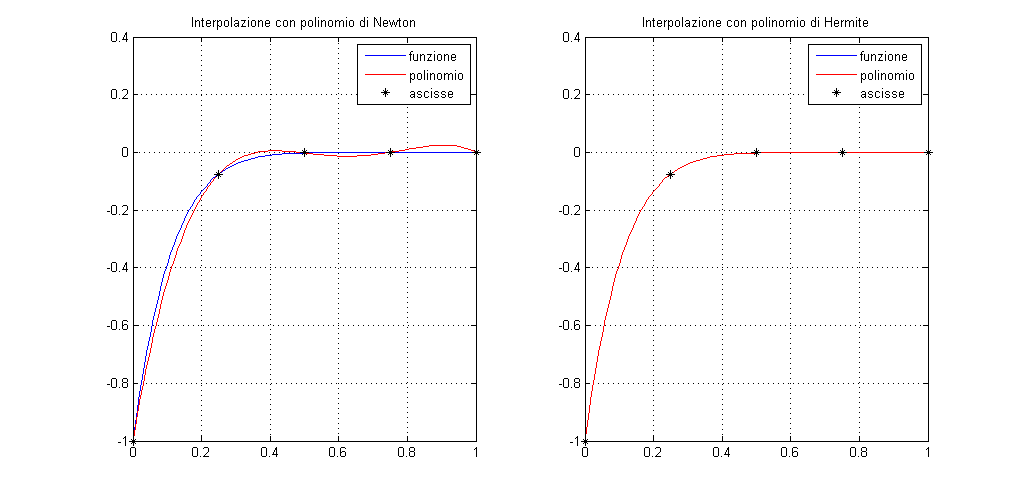
\includegraphics[scale=0.45]{img/es4_9a.png}
	\end{center}
	\begin{center}
		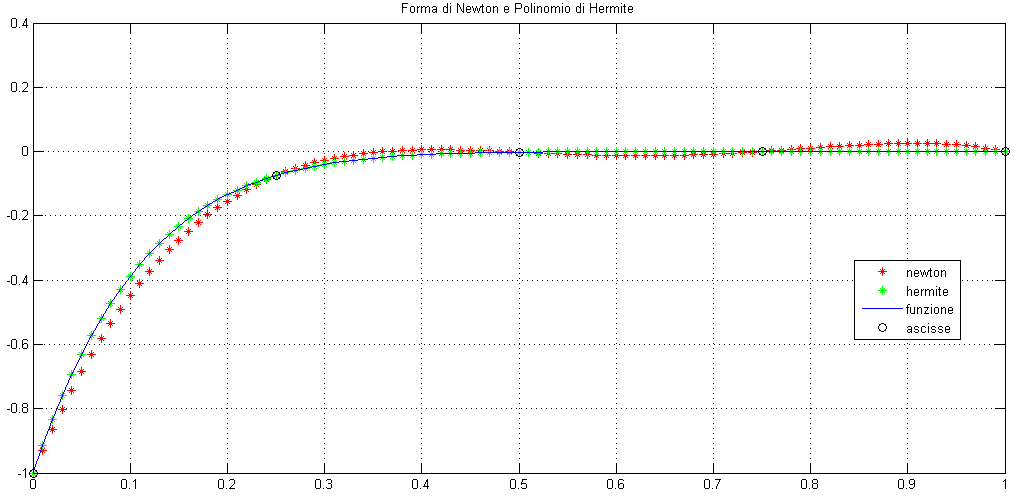
\includegraphics[scale=0.45]{img/es4_9b.png}
	\end{center}
	Dai grafici ottenuti si vede che l'interpolazione tramite polinomio di Newton approssima abbastanza bene
	la funzione, mentre utilizzando il polinomio di Hermite si ha una totale coincidenza tra la funzione originaria
	ed il polinomio interpolante. Questo è dovuto al fatto che il polinomio di Hermite interpola la funzione
	su un totale di $10$ ascisse, il che lo rende a tutti gli effetti un polinomio di grado $9$, esattamente
	come la funzione originaria.
	Il polinomio di newton, invece, interpolando la funzione su $5$ sole ascisse, risulta essere un polinomio di quarto grado.
	\lstinputlisting[caption={Esercizio \ref{es:4.9}.}, label=lst:es4.9]{code/es4_9.m}
\end{sol}
\sectionline{black}{88}

\section{Esercizio 10}
\label{sub:Esercizio 10}
\emph{Quante ascisse di interpolazione equidistanti sono necessarie per approssimare la funzione $\sin(x)$ sull'intervallo $[0,2\pi]$, con un errore di interpolazione inferiore a $10^{-6}$?}
\begin{sol}
	Sapendo che
	\[e(x)={\frac{f\textsuperscript{(n+1)}(\xi)}{(n+1)!}}w_{n+1}(x)\]
	vengono fatte le seguenti maggiorazioni:
	\[w_{n+1}(x)=\prod\limits_{i=1}^n (x-x_{i}) \leq \prod\limits_{i=1}^n (b-a) = (b-a)\textsuperscript{n}\]
	con $f\textsuperscript{(i)}(x) \leq 1 \forall{i=1,...n+1}$.
	Da cui segue:
	\[10\textsuperscript{-6} \leq \frac{1\text{}(b-a)\textsuperscript{n}}{(n-1)!} = \frac{2\pi\textsuperscript{n}}{(n-1)!}\]
	Dopo una serie tentativi su Matlab è stato ottenuto il seguente risultato n = 24.

	\lstinputlisting[caption={Esercizio \ref{es:4.10}.}, label=lst:es4.10]{code/es4_10.m}
\end{sol}
\sectionline{black}{88}

\section{Esercizio 11}
\label{sub:Esercizio 11}
\emph{Verificare sperimentalmente che, considerando le ascisse di interpolazione equidistanti (\ref{ascisseEquidistanti}) su cui si definisce il polinomio $p(x)$ interpolante $f(x)$, l'errore $||f-p||$ diverge, al crescere di $n$, nei seguenti due casi:}
			\begin{enumerate}
				\item \emph{esempio di Runge}:
					$$f(x)=\frac{1}{1+x^2},\qquad [a,b]\equiv[-5,5];$$
				\item \emph{esempio di Bernstein}:
					$$f(x)=|x|,\qquad [a,b]\equiv[-1,1].$$
			\end{enumerate}
\begin{sol}
	\begin{itemize}
		\item \underline{Esempio di Runge:}\\
			Osserviamo i seguenti grafici che mostrano, rispettivamente, l'errore commesso con $n=5,10,15$ e l'interpolazione della funzione per $n=5,10,15,20$:
			\begin{center}
				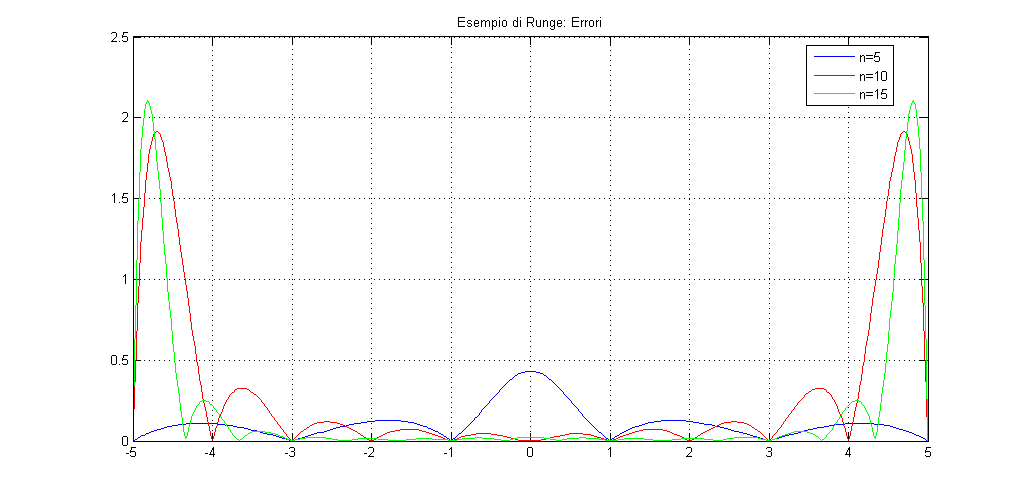
\includegraphics[scale=0.4]{img/es4_11a.png}
			\end{center}
			\begin{center}
				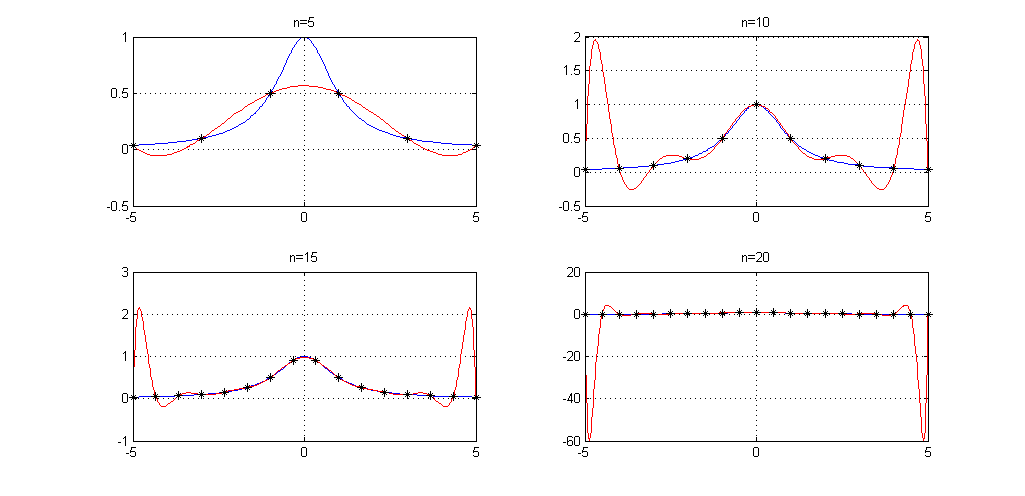
\includegraphics[scale=0.4]{img/es4_11b.png}
			\end{center}
		\item \underline{Esempio di Bernstein:}
			Come per l'esempio di Runge, proponiamo i grafici dell'errore e dell'interpolazione per l'esempio di Bernstein:
			\begin{center}
				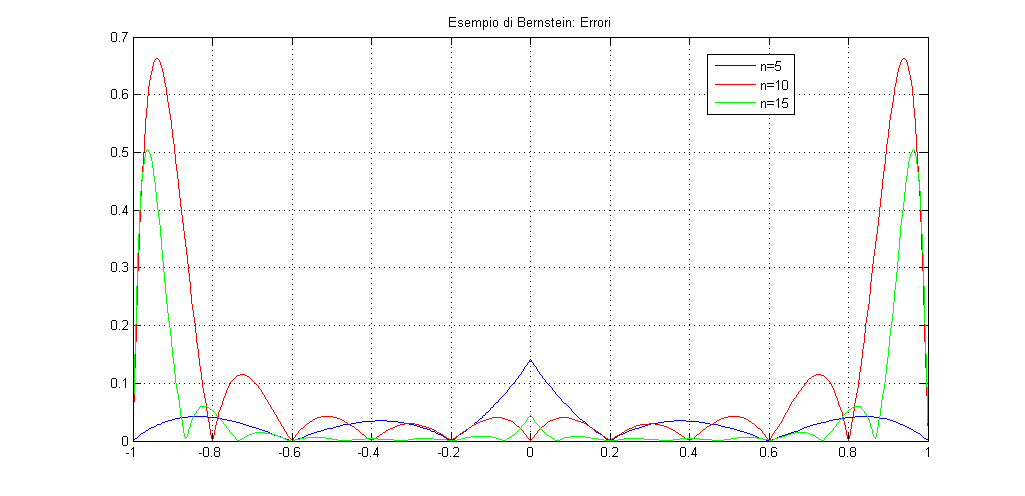
\includegraphics[scale=0.4]{img/es4_11c.png}
			\end{center}
			\begin{center}
				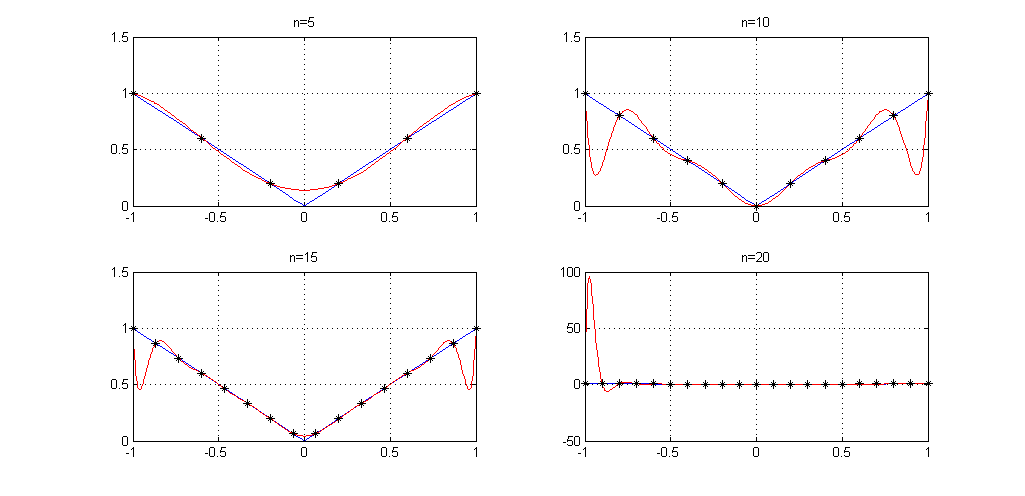
\includegraphics[scale=0.4]{img/es4_11d.png}
			\end{center}
	\end{itemize}
	Da i grafici proposti per le due funzioni d'esempio deduciamo che l'errore commesso tende a divergere all'aumentare di $n$ con le ascisse di interpolazione scelte equidistanti, ovvero uniformemente distribuite sull'intervallo di interpolazione. Vediamo infine i valori dell'errore massimo di interpolazione commesso nei due esempi per $n=5,10,15,20$:
	\begin{center}
		\begin{tabular}{c||c|c}
			\multirow{2}{*}{$n$} & \multicolumn{2}{|c}{\textbf{Errore}}\\
			& \textbf{Runge} & \textbf{Bernstein}\\
			\hline
			$5$ & 0.4327 & 0.0422\\
			$10$ & 0.3276 & 0.1149\\
			$15$ & 2.1076 & 0.5054\\
			$20$ & 59.8223 & 95.1889
		\end{tabular}
	\end{center}

	\lstinputlisting[caption={Esercizio \ref{es:4.11}.}, label=lst:es4.11]{code/es4_11.m}

\end{sol}
\sectionline{black}{88}

\section{Esercizio 12}
\label{sub:Esercizio 12}
\emph{Dimostrare che, se $x\in[-1,1]$, allora:
			$$\tilde{x}\equiv\frac{a+b}{2}+\frac{b-a}{2}x\in[a,b].$$
			Viceversa, se $\tilde{x}\in[a,b]$, allora:
			$$x\equiv\frac{2\tilde{x}-a-b}{b-1}\in[-1,1].$$
			Concludere che è sempre possibile trasformare il problema di interpolazione (4.1)-(4.2) in uno definito sull'intervallo $[-1,1]$, e viceversa.
}
\begin{sol}
	\normalfont
	\begin{itemize}
		\item $x\in[-1,1]\:\Rightarrow\:\tilde{x}\in[a,b]$:
	\begin{itemize}
		\item se $x=-1$, $\tilde{x}=\frac{a+b}{2}-\frac{b-a}{2} = a$;
		\item se $x=1$, $\tilde{x}=\frac{a+b}{2}+\frac{b-a}{2} = b$.
	\end{itemize}
		\item $\tilde{x}\in[a,b]\:\Rightarrow\:x\in[-1,1]$:
	\begin{itemize}
		\item se $\tilde{x}=a$, $x=\frac{2a-a-b}{b-a}=-1$;
		\item se $\tilde{x}=b$, $x=\frac{2b-a-b}{b-a}=1$;
	\end{itemize}
	\end{itemize}
\end{sol}

\sectionline{black}{88}

\section{Esercizio 13}
\label{sub:Esercizio 13}
\emph{Dimostrare le proprietà dei polinomi di Chebyshev di I specie (4.24) elencate nel Teorema 4.9.
}
\begin{sol}
	\normalfont
	Prime proprietà
	\begin{enumerate}
		\item $T_k(x)$ è un polinomio di grado esatto $k$:
	\begin{itemize}
		\item $k=0$: $T_0(x)=1$ polinomio di grado $0$;
		\item $k>0$: $T_{k+1}(x)=2xT_k(x)-T_{k-1}(x)$ dove, per ipotesi induttiva, $T_k(x)$ è un polinomio di grado $k$ quindi $T_{k+1}(x)$ è un polinomio di grado $k+1$.
	\end{itemize}
		\item Il coefficiente principale di $T_k(x)$ è $2^{k-1}$, $k=1,2,\ldots$:
		\begin{itemize}
		\item $k=1$: $T_1(x)=x$ e $2^{1-1}=1$;
		\item $k>1$: $T_{k+1}(x)=2xT_k(x)-T_{k-1}(x)$ dove, per ipotesi induttiva, il coefficiente principale di $T_k(x)$ è $2^{k-1}$ quindi il coefficiente principale di $T_{k+1}(x)$ è $2\cdot2^{k-1}=2^k$.
	\end{itemize}
		\item La famiglia di polinomi $\{\hat{T}_k\}$, in cui $$\hat{T}_0(x)=T_0(x),\quad\hat{T}_k(x)=2^{1-k}T_k(x),\quad k=1,2,\ldots,$$ è una famiglia di polinomi monici di grado $k$, $k=1,2,\ldots$:
	\begin{itemize}
		\item grado $k$: il grado di $\hat{T}_k$ coincide con il grado di $T_k(x)$ che è $k$;
		\item monici: il coefficiente principale di $\hat{T}_k$ è $2^{1-k}$ dunque $2^{1-k}2^{k-1}=1$ il polinomio è monico.
	\end{itemize}
		\item Ponendo $x=\cos{\theta}$, $\theta\in[0,\pi]$, si ottiene $T_k(x)=T_k(\cos{\theta})=\cos{k\theta},\quad k=0,1,\ldots$:
	\begin{itemize}
		\item $k=0$: $T_0(\cos{\theta})=\cos{0\theta}=1=T_0(x)$;
		\item $k=1$: $T_0(\cos{\theta})=\cos{\theta}=x=T_1(x)$:
		\item $k>1$: $T_{k+1}(\cos{\theta})=2\cos{\theta}T_k({\cos{\theta}})-T_{k-1}(\cos{\theta})$ per ipotesi induttiva, $T_k({\cos{\theta}})=\cos{k\theta}$ e $T_{k-1}(\cos{\theta})=\cos{(k-1)\theta}$ dunque $T_{k+1}(\cos{\theta})=2\cos{\theta}\cos{k\theta}-\cos{(k-1)\theta}=\cos{(k+1)\theta}+\cos{(k-1)\theta}-\cos{(k-1)\theta}=\cos{(k+1)\theta}=T_{k+1}(x)$.
	\end{itemize}
	\end{enumerate}
	Teorema 4.9
	\begin{itemize}
		\item Radici del polinomio: $T_k(x)=T_k(\cos{\theta})=\cos{k\theta}=0$ se $\cos{k\theta}=0$ ovvero per $k\theta=\frac{\pi}{2}+i\pi$; segue $\theta_i=\frac{\frac{\pi}{2}+i\pi}{k}=\frac{(2i+1)\pi}{2k}$ cioè gli zeri del polinomio sono dati da $x_i^{(k)}=\cos{\frac{(2i+1)\pi}{2k}}$.
		\item Estremi: Agli estremi $\cos{k\theta}=\pm 1$ ovvero $k\theta=i\pi$; segue $\theta_i=\frac{i}{k}\pi$ dunque gli estremi sono assunti in $\xi_i^{(k)}=\cos{\frac{i}{k}\pi}$; in tali punti, poiché $\cos{k\pi}=(-1)^i$ la funzione vale $T_k(\xi_i^{(k)})=(-1)^i$.
		\item Norme: dal punto precedente segue inoltre $||T_k||=1$ e  $||\hat{T}_k||=||2^{1-k}T_k||=||2^{1-k}||$.
		\item Minima norma per $\hat{T}_k(x)$: supponiamo per assurdo che $\exists p\neq\hat{T}_k(x)$ monico tale che $||p||<2^{1-k}=||\hat{T}_k||$, quindi $g(x)=\hat{T}_k-p(x)\in\Pi_{k-1}$ poiché entrambi monici di grado $K$. Studiando il segno di $g$ si nota $sign(g(x_i))=(-1)^i$ per $i=0,\ldots,k$ ovvero ci sono $k$ cambiamenti di segno quindi $k$ radici cioè $g(x)\in\Pi_k$ ma, per ipotesi, $g(x)\in\Pi_{k-1}$ quindi $g(x)=0$.
	\end{itemize}
\end{sol}

\sectionline{black}{88}

\section{Esercizio 14}
\label{sub:Esercizio 14}
\emph{Quali diventano le ascisse di Chebyshev (4.26), per un problema definito su un generico intervallo $[a,b]$?}
\begin{sol}
	Nel caso a=-1 e b=1, la formula per il calcolo delle ascisse di Chebyshev è:
	$x_{i}^{(k)}=cos(\frac{(2i+1)\pi}{2k})$  con k grado del polinomio e $i=0,...,k$.

	Nel caso generico, la formula diventa:
	$x_{i}^{(k)}=\frac{a+b}{2}+\frac{b-a}{2}cos(\frac{(2i+1)\pi}{2k})$  con k grado del polinomio e $i=0,...,k$.
\end{sol}

\sectionline{black}{88}

\section{Esercizio 15}
\label{sub:Esercizio 15}
\emph{Utilizzare le ascisse di Chebyshev (4.26) per approssimare gli esempi visti nell'Esercizio 4.11, per $n=2,4,6,\dots,40$.}
\begin{sol}
	Similmente a quanto visto nell'Esercizio 4.11 mostriamo di seguito i grafici degli errori e di interpolazione per $n=5,10,15,20$,
	rispetto agli esempi di Runge e Bernstein.
	\begin{itemize}
		\item \underline{Esempio di Runge}:
			\begin{center}
				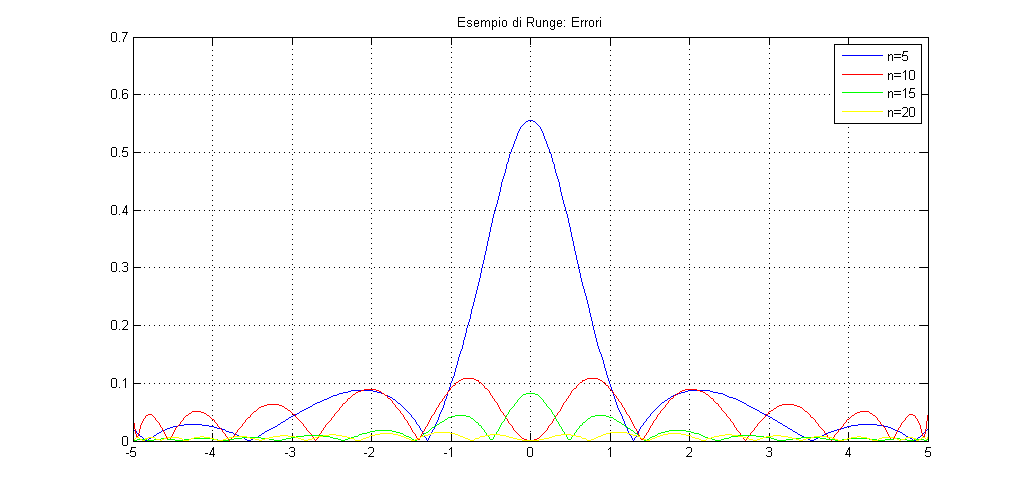
\includegraphics[scale=0.4]{img/es4_15a.png}
			\end{center}
			\begin{center}
				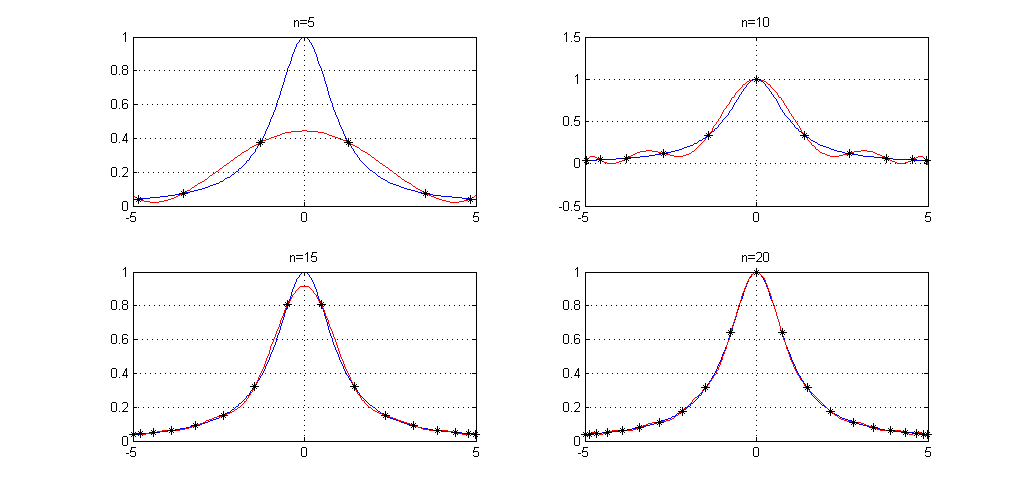
\includegraphics[scale=0.4]{img/es4_15b.png}
			\end{center}
		\item \underline{Esempio di Bernstein}:
			\begin{center}
				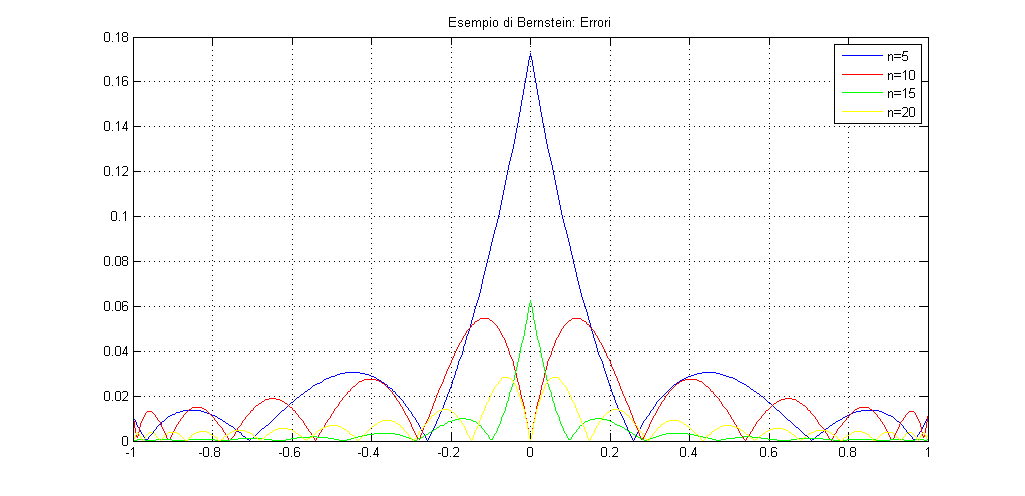
\includegraphics[scale=0.4]{img/es4_15c.png}
			\end{center}
			\begin{center}
				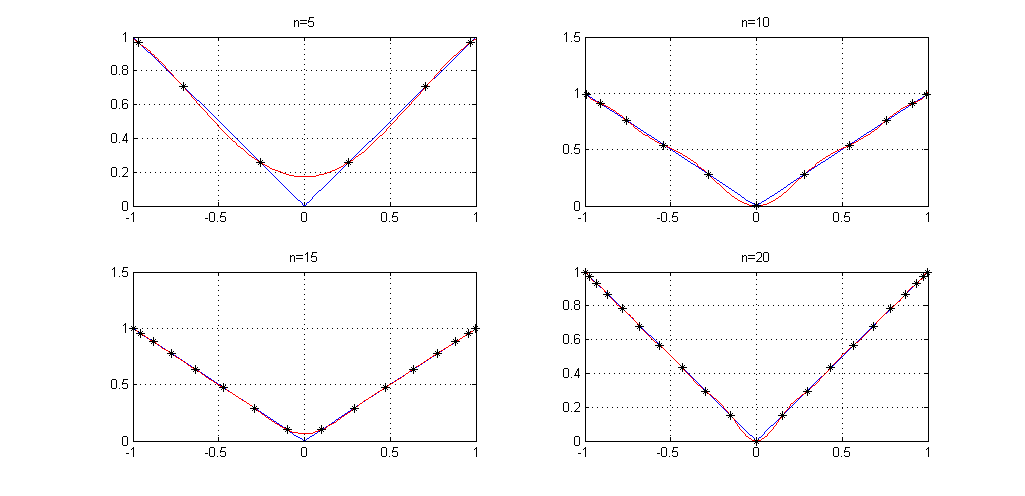
\includegraphics[scale=0.4]{img/es4_15d.png}
			\end{center}
	\end{itemize}
	Di seguito proponiamo anche gli errori di interpolazione massimi commessi nei due esempi per $n=5,10,15,20$:
	\begin{center}
		\begin{tabular}{c||c|c}
			\multirow{2}{*}{$n$} & \multicolumn{2}{|c}{\textbf{Errore}}\\
			& \textbf{Runge} & \textbf{Bernstein}\\
			\hline
			$5$ & 0.0881 & 0.0305\\
			$10$ & 0.0897 & 0.0275\\
			$15$ & 0.0831 & 0.0628\\
			$20$ & 0.0153 & 0.0140
		\end{tabular}
	\end{center}
	Si evince quindi, dai grafici e dai valori riportati,
	che la scelta delle ascisse di Chebyshev al posto di ascisse equidistanti è estremamente più conveniente,
	in quanto evita la divergenza dell'errore di interpolazione all'aumentare di $n$. Infatti l'errore commesso,
	all'aumentare di $n$ risulta essere in generale molto stabile e, molto spesso, risulta anche in diminuzione.

	\lstinputlisting[caption={Esercizio \ref{es:4.15}.}, label=lst:es4.15]{code/es4_15.m}

\end{sol}
\sectionline{black}{88}

\section{Esercizio 16}
\label{sub:Esercizio 16}
\emph{Verificare che la fattorizzazione $LU$ della matrice dei coefficienti del sistema tridiagonale (4.40) è dato da:}
			\[
				L=
				\begin{pmatrix}
					1 & & &\\
					l_2 & 1 & &\\
					& \ddots & \ddots &\\
					& & l_{n-1} & 1
				\end{pmatrix},
				\qquad U=
				\begin{pmatrix}
					u_1 & \xi_1 & &\\
					& u_2 & \ddots &\\
					& & \ddots & \xi_{n-2}\\
					& & & u_{n-1}
				\end{pmatrix},
			\]
			con
			\begin{align*}
				&u_1=2,\\
				&l_i=\frac{\varphi_i}{u_{i-1}},\\
				&u_i=2-l_i\xi_{i-1},\qquad i=2,\dots,n-1.
			\end{align*}
\emph{Scrivere una \lstinline{function} \textsc{Matlab} che implementi efficientemente la risoluzione della (4.40).}
\begin{sol}
	La matrice dei coefficienti
	\[
		A=\begin{pmatrix}
			2 & \xi_1 & & &\\
			\varphi_2 & 2 & \xi_2 & &\\
			& \ddots & \ddots & \ddots &\\
			& & \ddots & \ddots & \xi_{n-2}\\
			& & & \varphi_{n-1} & 2
		\end{pmatrix}
	\]
	si vede essere \textit{dominante per righe} in quanto, essendo
	$$\varphi_i=\frac{h_i}{h_i+h_{i+1}},\qquad\xi_i=\frac{h_{i+1}}{h_i+h_{i+1}},\qquad i=1,\dots,n-1,$$
	si vede facilmente che $\varphi_i+\xi_i=1$. Quindi la matrice è fattorizzabile $LU$.\\
	Moltiplichiamo adesso i termini $L$ ed $U$ e vediamo che il risultato sono proprio i termini della matrice $A$:
	\begin{itemize}
		\item $a_{11}=1\cdot u_1=u_1=2$;
		\item $a_{12}=1\cdot\xi_1 + 0\cdot u_2=\xi_1$;
		\item $a_{i,i-1}=0\cdot\xi_{i-2}+l_i\cdot u_{i-1}+1\cdot 0=l_i\cdot u_{i-1}=\frac{\varphi_i}{u_{i-1}}u_{i-1}=\varphi_i$, per $i>1$;
		\item $a_{ii}=l_i\cdot\xi_{i-1}+1\cdot u_i=l_i\xi_{i-1}+2-l_i\xi_{i-1}=2$, per $i>1$;
		\item $a_{i,i+1}=l_i\cdot 0+1\cdot\xi_i +0\cdot u_{i+1}=\xi_i$, per $i>1$.
	\end{itemize}
	Quindi il sistema $A\underline{m}=\underline{d}$ si risolve come segue:
	\begin{itemize}
		\item si risolve $L\underline{y}= 6\underline{d}$:
			\begin{itemize}
				\item $y_1=6d_1$,
				\item $y_i=6d_i-l_iy_{i-1}$ per $i=2,\dots,n-1$;
			\end{itemize}
		\item si risolve il sistema $U\underline{m}=\underline{y}$:
			\begin{itemize}
				\item $m_{n-1}=\frac{y_{n-1}}{u_{n-1}}$,
				\item $m_{i}=\frac{y_i-\xi_i m_{i+1}}{u_i}$, per $i=n-2, \dots ,1$.
			\end{itemize}
	\end{itemize}
	\lstinputlisting[caption={Calcolo dei fattori $\{m_i\}$ per una \textit{spline} cubica naturale.}, label=lst:risolviSistemaSplineNaturale]{code/risolviSistemaSplineNaturale.m}
\end{sol}

\sectionline{black}{88}

\section{Esercizio 17}
\label{sub:Esercizio 17}
\emph{Generalizzare la fattorizzazione del precedente Esercizio 4.16 al caso della matrice dei coefficienti del sistema lineare
(4.41). Scrivere una corrispondente \lstinline{function} \textsc{Matlab} che risolva efficientemente questo sistema.
}
\begin{sol}
	Generalizzando il risultato ottenuto nell'Esercizio 4.16, la fattorizzazione è della forma
	\[
		L=\begin{pmatrix}
			1 & & &\\
			l_2 & 1 & &\\
			& \ddots & \ddots &\\
			& & l_{n+1} & 1
		\end{pmatrix},\qquad U=\begin{pmatrix}
			u_1 & w_1 & &\\
			& u_2 & \ddots &\\
			& & \ddots & w_n\\
			& & & u_{n+1}
		\end{pmatrix}.
	\]
	Se come prima moltiplichiamo i fattori $L$ ed $U$ ricaviamo le espressioni degli $l_i$, $u_i$ e $w_i$:
	\begin{itemize}
		\item per $i=4,\dots,n-1$:
			\[
				\begin{cases}
					u_i=2-l_iw_{i-1}\\
					w_{i-1}=\xi_{i-2}\\
					l_i=\frac{\varphi_{i-1}}{u_{i-1}}
				\end{cases};
			\]
		\item per $i=3$:
			\[
				\begin{cases}
					u_3=2-l_3w_2\\
					w_2=\xi_1-\varphi_1\\
					l_3=\frac{\varphi_2}{u_2}
				\end{cases};
			\]
		\item per $i=2$:
			\[
				\begin{cases}
					u_2=2-\varphi_1\\
					w_1=0\\
					l_2=\frac{\varphi_1}{u_1}
				\end{cases};
			\]
		\item per $i=1$:
			$$u_1=1;$$
		\item per $i=n$:
			\[
				\begin{cases}
					u_n=2-\xi_{n-1}-l_nw_{n-1}\\
					w_{n-1}=\xi_{n-2}\\
					l_n=\frac{\varphi_{n-1}-\xi_{n-1}}{u_{n-1}}
				\end{cases};
			\]
		\item per $i=n+1$:
			\[
				\begin{cases}
					u_{n+1}=1\\
					w_n=\xi_{n-1}\\
					l_{n+1}=0
				\end{cases}
			\].
	\end{itemize}
	Quindi come prima avremo:
	\begin{itemize}
		\item risoluzione del sistema $L\underline{y}= 6\underline{d}$:
			\begin{itemize}
				\item $y_1=6d_1$,
				\item $y_i=6d_i-l_iy_{i-1}$ per $i=2,\dots,n+1$;
			\end{itemize}
		\item risoluzione del sistema $U\underline{\hat{m}}=\underline{y}$:
			\begin{itemize}
				\item $\hat{m}_{n+1}=\frac{y_{n+1}}{u_{n+1}}$,
				\item $\hat{m}_{i}=\frac{y_i-w_i \hat{m}_{i+1}}{u_i}$, per $i=n, \dots ,1$;
			\end{itemize}
		\item calcolo della soluzione:
			\begin{itemize}
				\item $m_1=\hat{m}_1-\hat{m}_2-\hat{m}_3$,
				\item $m_i=\hat{m}_i$, per $i=2,\dots,n$,
				\item $m_{n+1}=\hat{m}_{n+1}-\hat{m}_n-\hat{m}_{n-1}$.
			\end{itemize}
	\end{itemize}
	Qui si propone il codice:\\
	\lstinputlisting[caption={Calcolo dei fattori $\{m_i\}$ per una \textit{spline} cubica \textit{not-a-knot}.}, label=lst:risolviSistemaSplineNotAKnot]{code/risolviSistemaSplineNotAKnot.m}
\end{sol}
\sectionline{black}{88}

\section{Esercizio 18}
\label{sub:Esercizio 18}
\emph{Scrivere una \lstinline{function} \textsc{Matlab} che, noti gli $\{m_i\}$ in (4.32), determini l'espressione,
polinomiale a tratti, della spline cubica (4.36).}
\begin{sol}
	\lstinputlisting[caption={Calcolo delle espressioni di una \textit{spline} (noti i fattori $\{m_i\}$).}, label=lst:espressioniSplineCubica]{code/espressioniSplineCubica.m}
\end{sol}

\sectionline{black}{88}

\section{Esercizio 19}
\label{sub:Esercizio 19}
\emph{Costruire una \lstinline{function} \textsc{Matlab} che implementi le spline cubiche naturali e quelle definite dalle condizioni not-a-knot.
}
\begin{sol}
	\lstinputlisting[caption={Calcolo delle espressioni di una \textit{spline} (naturale o con condizioni \textit{not-a-knot}).}, label=lst:splineCubica]{code/splineCubica.m}
\end{sol}
\sectionline{black}{88}

\section{Esercizio 20}
\label{sub:Esercizio 20}
\emph{Utilizzare la \lstinline{function} dell'Esercizio 4.19 per approssimare,
su partizioni (4.28) uniformi con $n=10,20,30,40$, gli esempi proposti nell'Esercizio 4.11.}
\begin{sol}
	I grafici ottenuti mostrano l'interpolazione delle due funzioni d'esempio tramite spline cubiche con condizioni \textit{not-a-knot} (si osservi che nei grafici i due punti definiti, appunto, \textit{not-a-knot}, sono indicati da un cerchio nero al posto di un asterisco come per tutti gli altri nodi). Non sono stati riportati i grafici riguardanti l'interpolazione tramite spline cubiche naturali in quanto tra i due tipi di grafici non sono presenti sostanziali differenze (eseguendo il file \textsc{Matlab} relativo vengono disegnati entrambi i grafici per i due esempi).
	\begin{itemize}
		\item \underline{Esempio di Runge}:
			\begin{center}
				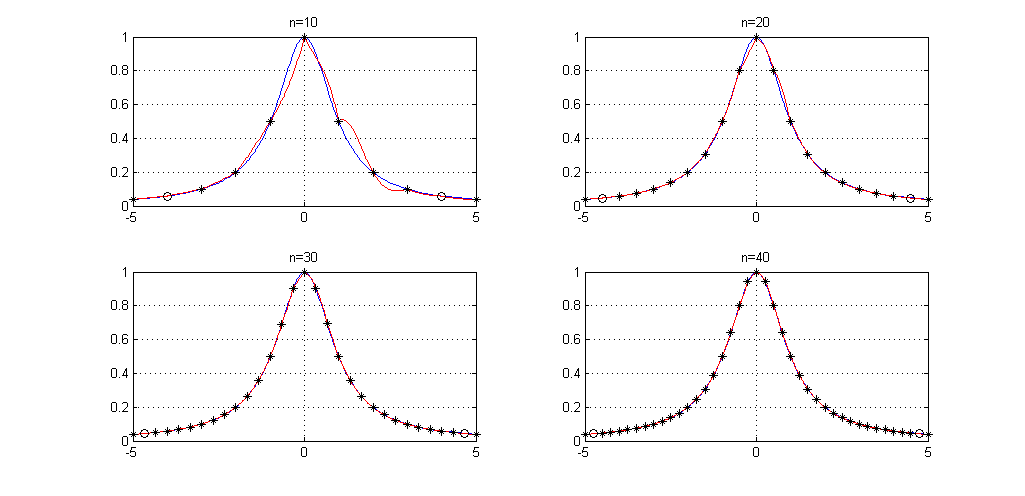
\includegraphics[scale=0.4]{img/es4_20a.png}
			\end{center}
		\item \underline{Esempio di Bernstein}:
			\begin{center}
				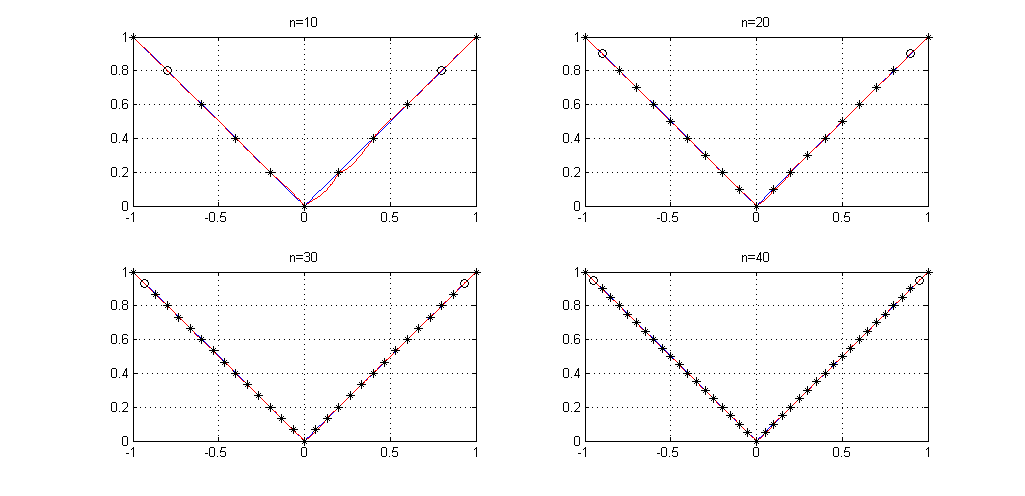
\includegraphics[scale=0.4]{img/es4_20b.png}
			\end{center}
	\end{itemize}
	Qui si propone il codice:\\
	\lstinputlisting[caption={Esercizio \ref{es:4.20}.}, label=lst:es4.20]{code/es4_20.m}
\end{sol}
\sectionline{black}{88}

\section{Esercizio 21}
\label{sub:Esercizio 21}
\emph{Interpretare la retta dell'Esercizio 3.32 come retta di approssimazione ai minimi quadrati dei dati.}
\begin{sol}
	\normalfont Il problema ai minimi quadrati è dato da
	$$\min_{a_1,a_2\in\mathbb{R}}{\sum_{k=0}^n{|y_i-a_1x_i-a_2|^2}}$$
	dove $\underline{y}$ è il vettore dei valori previsti per la retta.
	Il problema è esprimibile in forma matriciale come
	$$\begin{pmatrix}1&x_0\\1&x_1\\\vdots&\vdots\\1&x_n\end{pmatrix}\begin{pmatrix}a_2\\a_1\end{pmatrix}=\begin{pmatrix}y_0\\y_1\\\vdots\\y_n\end{pmatrix} ;$$
	si tratta di risolvere un sistema sovradeterminato che ha soluzione se almeno $2$ ascisse sono distinte in quanto $r(x)\in\Pi_1$.
\end{sol}
\sectionline{black}{88}

\section{Esercizio 22}
\label{sub:Esercizio 22}
\emph{È noto che un fenomeno ha un decadimento esponenziale, modellizzato come}
			$$y=\alpha\cdot e^{-\lambda t},$$
			in cui $\alpha$ e $\lambda$ sono parametri positivi e incogniti. Riformulare il problema in modo che il modello sia di tipo polinomiale. Supponendo inoltre di disporre delle seguenti misure,
			\begin{center}
				\setlength{\tabcolsep}{4pt}
				\begin{tabular}{|c|c c c c c c c c c c c|}
					\hline
					$t_1$ & 0 & 1 & 2 & 3 & 4 & 5 & 6 & 7 & 8 & 9 & 10\\
					\hline
					$y_i$ & 5.22 & 4.00 & 4.28 & 3.89 & 3.53 & 3.12 & 2.73 & 2.70 & 2.20 & 2.08 & 1.94\\
					\hline
				\end{tabular}
			\end{center}
\emph{calcolare la stime ai minimi quadrati dei due parametri incogniti. Valutare il residuo e raffigurare, infine, i risultati ottenuti.}
\begin{sol}
	\normalfont
	Il problema in forma polinomiale è
	$$\bar{y}=\bar{\alpha}+\bar{\lambda}t,\quad\mbox{ con }\bar{y}=\log{y}\mbox{, }\bar{\alpha}=\log{\alpha}\mbox{ e }\bar{\lambda}=-\lambda$$
	infatti si ha
	$y=\alpha\cdot e^{-\lambda t}\:\Rightarrow\:\log{y}=\log{(\alpha\cdot e^{-\lambda t})}\:\Rightarrow\:\log{y}=\log{\alpha}-\lambda t\:\:\Rightarrow\:\bar{y}=\bar{\alpha}+\bar{\lambda}t$.
	Si tratta di risolvere il sistema lineare sovradeterminato $$\begin{pmatrix}1&t_0\\1&t_1\\\vdots&\vdots\\1&t_10\end{pmatrix}\begin{pmatrix}\bar{\alpha}\\\bar{\lambda}\end{pmatrix}=\begin{pmatrix}\bar{y}_0\\\bar{y}_1\\\vdots\\\bar{y}_n\end{pmatrix}$$
	mediante fattorizzazione $QR$ (possibile poiché tutte le ascisse sono distinte) e ricavare $\begin{pmatrix}\bar{\alpha}\\\bar{\lambda}\end{pmatrix}$ da qui $\begin{pmatrix}\alpha\\\lambda\end{pmatrix}=\begin{pmatrix}e^{\bar{\alpha}}\\-\bar{\lambda}\end{pmatrix}.$\\
	I risultati ottenuti dallo \lstinline{scritp} \textsc{Matlab} sono $\begin{pmatrix}\alpha\\\lambda\end{pmatrix}=\begin{pmatrix}5.008\\0.0959\end{pmatrix}$ con un residuo $r=0.1708$. \centering\begin{figure}[H]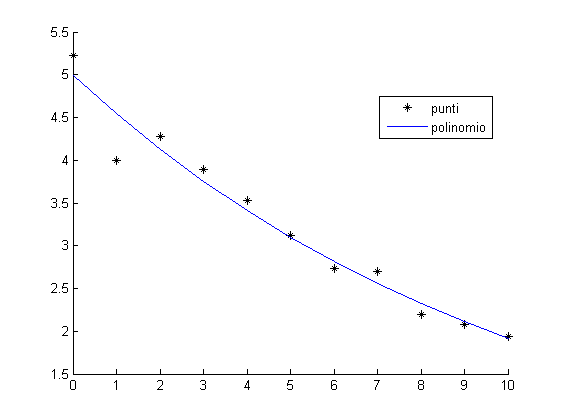
\includegraphics[scale=0.60]{img/es4_22.png}\end{figure}
	Qui si propone il codice:\\
	\lstinputlisting[caption={Esercizio \ref{es:4.22}.}, label=lst:es4.22]{code/es4_22.m}
\end{sol}
